%%%%%%%%%%%%%%%%%%%%%%%%%%%%%%%%%%%%%%%%%%%%%%%%%%%%%%%%%%%%%%%%%%%%%%%%%%%%%%%%%%%%%%%%%%%%%%%%%%%%%%%%%%%%%%%%%%%%%%%%%%%%%%%%%%%%%%%%
% This is just a template to use when submitting manuscripts to Frontiers, it is not mandatory to use frontiers.cls nor frontiers.tex  %
%%%%%%%%%%%%%%%%%%%%%%%%%%%%%%%%%%%%%%%%%%%%%%%%%%%%%%%%%%%%%%%%%%%%%%%%%%%%%%%%%%%%%%%%%%%%%%%%%%%%%%%%%%%%%%%%%%%%%%%%%%%%%%%%%%%%%%%%

\documentclass{frontiersSCNS} % for Science articles
%\documentclass{frontiersMED} % for Medicine articles

\usepackage{url}
\usepackage{lineno}

\usepackage{todonotes}

\newcommand{\alex}[1]{\todo[inline, color=green!40]{#1}}



\linenumbers


\copyrightyear{}
\pubyear{}
%\onecolumn
%%% write here for which journal %%%
\def\journal{Neurosciences}
\def\DOI{}
\def\articleType{}
\def\citing{\color{darkgray}\cite}
\def\keyFont{\fontsize{6}{11}\helveticabold }
\def\firstAuthorLast{Sample {et~al}} %use et al only if is more than 1 author
\def\Authors{Alexandre Abraham\,$^{1,2,*}$, Fabian Pedregosa\,$^{1,2}$, Andreas Muller, Jean Kossaifi, Philippe Gervais\,$^{1,2}$, Alexandre Gramfort, Bertrand Thirion\,$^{1,2}$ and Gaël Varoquaux\,$^{1,2}$}
% Affiliations should be keyed to the author's name with superscript numbers and be listed as follows: Laboratory, Institute, Department, Organization, City, State abbreviation (USA, Canada, Australia), and Country (without detailed address information such as city zip codes or street names).
% If one of the authors has a change of address, list the new address below the correspondence details using a superscript symbol and use the same symbol to indicate the author in the author list.
\def\Address{
    $^{1}$Parietal Team, INRIA Saclay-\^{I}le-de-France, Saclay, France\\
    $^{2}$Neurospin, I\textsuperscript{2}BM, DSV, CEA, 91191 Gif-Sur-Yvette, France}

% The Corresponding Author should be marked with an asterisk
% Provide the exact contact address (this time including street name and city zip code) and email of the corresponding author
\def\corrAuthor{Alexandre Abraham}
\def\corrAddress{Parietal Team, INRIA Saclay-\^{I}le-de-France, Saclay, France}
\def\corrEmail{alexandre.abraham@inria.fr}

% \color{FrontiersBlue} Is the blue color, used in the Journal name, in the title, and the names of the sections


% Example of table from template

% \begin{table}[!t]
% \processtable{Resolution Requirements for the figures\label{Tab:01}}
% {\begin{tabular}{lllll}\toprule
% Image Type & Description & Format & Color Mode & Resolution\\\midrule
% Line Art & An image composed of lines and text,  & TIFF, EPS, JPEG & RGB, Bitmap & 900 - 1200 dpi\\
%            & which does not contain tonal or shaded areas.& & &\\
%            Halftone & A continuous tone photograph, which contains no text. & TIFF, EPS, JPEG & RGB, Grayscale & 300 dpi\\
% Combination & Image contains halftone + text or line art elements. & TIFF, EPS, JPEG & RGB,Grayscale & 600 - 900 dpi\\\botrule
% \end{tabular}}{This is a footnote}
% \end{table}


% Figures

% \textbf{Figure 1.}{ Enter the caption for your figure here.  Repeat as  necessary for each of your figures.}\label{fig:01}
% Don't add the figures in the LaTeX files, please upload them when submitting the article. Frontiers will add the figures at the end of the provisional pdf.



\begin{document}
\onecolumn
\firstpage{1}

\title[Running Title]{This is Title}
\author[\firstAuthorLast ]{\Authors}
\address{}
\correspondance{}
\editor{}
\topic{Research Topic}

\maketitle
\begin{abstract}

\section{}
Statistical  learning  methods  are   increasingly  used  to  perform
neuroimaging  analysis.  Their  main  virtue  for this  type  of  application
is  their  ability  to   model  high-dimensional  datasets,  e.g.\ multivariate
analysis  of activation  images,  or  capturing  inter­subject  variability.
Supervised  learning  is  typically  used  in  “decoding” setting  to  relate
brain   images  to  behavioral  or  clinical  observations,  while
unsupervised  learning  is  typically used  to  uncover  hidden  structure  in
sets  of  images   (e.g.\ resting  state  functional  MRI)  or  to  find
sub­populations  in  large  cohorts  of  subjects.   By  considering
functional  neuroimaging  use  cases,  we illustrate  how  the  Scikit­learn,
a  Python machine  learning  library,  can  be used to perform  some  key
analysis steps.  Scikit­learn  contains  a  large   set  of  statistical
learning  algorithms,  both  supervised  and unsupervised, that can be  applied
to neuroimaging data after a  proper preprocessing.  Combined  with  other
Python  libraries, neuroimaging data can be loaded, processed and the results
can be visualised easily.



\tiny
  \section{Keywords:} Text Text Text Text Text Text Text Text  %All article types: you may provide up to 8 keywords; at least 5 are mandatory.
\end{abstract}


\section{Introduction}


\subsection{Python scientific and neuroimaging ecosystem}

\subsubsection{Scipy and Numpy}
\subsubsection{nibabel}
\subsubsection{nipy}
\subsubsection{scikit-learn}



% Here we present the Python neuroimaging ecosystem : scikit­learn, nibabel,
% nipy.

\section{Scikit-learn concepts}

% Present the underlying concepts of scikit­learn: estimator,­ data
% representation, transformer...

\subsection{Estimator}

\subsection{Data representation}

Explain that the scikit process 2D data. This is an introduction to masking.

\subsection{Transformer}

\subsection{Pipeline}

Make a reference to SVM example

\subsection{Cross validation}

\alex{It seems more right to me to put it in this part}


\section{Datasets}

\alex{I think this should be good to talk about datasets from the beginning to
    introduce what we will want (introducing examples) and to be able to cite
    them from the beginning (we may want to precise what kind of preprocessing
is requirend on which dataset and why).}

\subsection{Haxby}

\subsection{Kamitani}

BOLD response is usually 4/6 seconds after the stimulus. For Kamitani, we shift
the stimuli by 2 TR.

\subsection{NYU Test-Retest}



\section{Preparing the data}

\subsection{Data Preparation}
    % or Signal Processing ?

% Neuroimaging  data  requires  special  preparation  due  to  its  particular
% nature  and acquisition  protocol (normalization, detrending...).

\subsection{Resampling}

\begin{itemize}
    \item Necessary for multi subjects (do we speak of this problem before ?)
    \item This is one way of decreasing data size
    \item Removing confounds is necessary for some treatments
\end{itemize}

\subsection{Signal cleaning}

\begin{itemize}
    \item Remove high frequency (scanner artefacts)
\end{itemize}

% I think that we should present the challenges about NI data here. Poor SNR,
% multi subject / session...

\subsection{Dimension reduction}

\begin{itemize}
    \item Data is often too big for computation, we need to reduce its
        dimensionality
\end{itemize}

\subsubsection{Resampling}

Resampling is a way to reduce dimensionality.

\subsubsection{Feature selection}

Speak of Anova here. This is one of the simplest way to reduce efficiently
dimensionality.

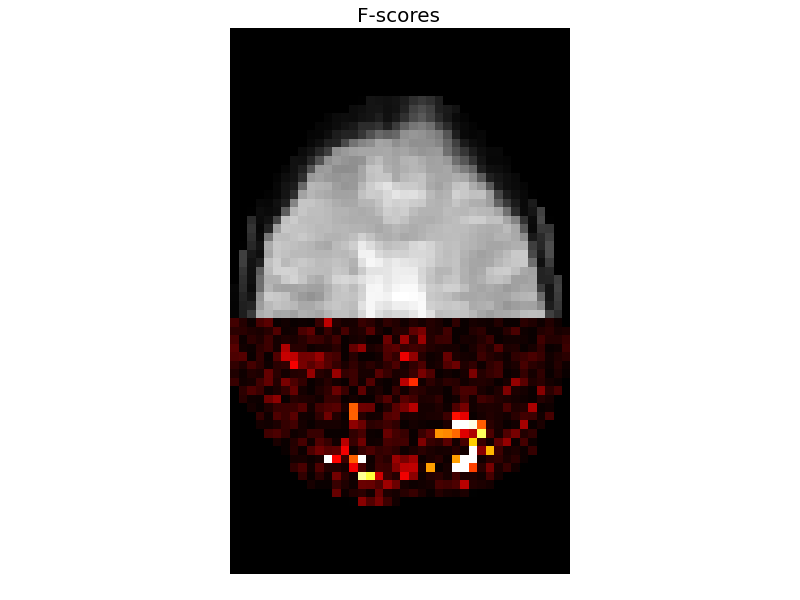
\includegraphics[width=.5\linewidth]{img/plot_haxby_searchlight_2.png}

\subsubsection{Clustering / ROI}

We can select regions to reduce dimensionality. For example, V1 for a visual
task. We can also segment automatically the brain thanks to a Ward, or use a
reference atlas.

\subsubsection{PCA}

The PCA is good to reduce dimensionality in the time series dimension (other
methods are for spatial reduction).


\subsection{Masking}

% This   step  turns  the  data  into  the  scikit­learn   compliant  formant
% n_features  x  n_samples.  We  may speak of connectivity graph that allow to
% integrate the 3D structure of the data in some algorithms.

\subsubsection{From 4-dimensional image to 2-dimensional array}

Neuroimaging data are represented in 4 dimensions: 3 dimensions for the scans,
which are positioned in a coordinate space, and one dimension for the time.
Scikit-learn algorithms, on the other hand, only accept 2-dimensional data: one
dimension for the features and one for the samples.\\

Consequently, in order to use neuroimaging data in the scikit-learn, a
conversion is needed. The most simple way to achieve that would be to
\emph{flatten} the 3D scans into a 1D array. However, we know that not every
voxels in a neuroimaging scan is useful. In particular, outter-brain voxels are
of no use and, worse, they can bring spurious noise and scanner artefacts (such
as ghosts).\\

To sort out voxels of interest, we will have to apply a mask on the data. Most
of public datasets provide a mask, come of them even provide several, isolating
different functional or anatomical brain regions. \alex{ref to Haxby}

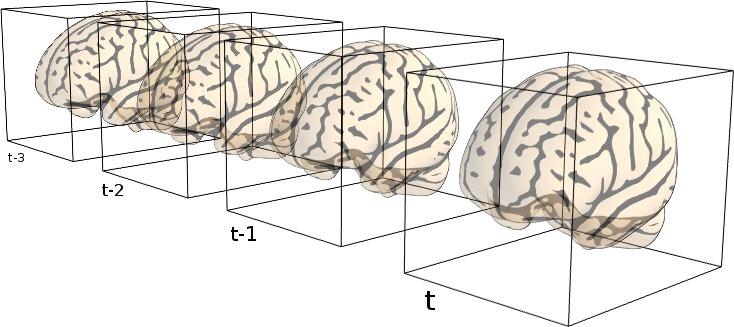
\includegraphics[width=.5\linewidth]{img/niimgs.jpg}

\alex{Should tell here that some algorithms, like logistic regression, do not
like colinear features.}

\subsubsection{Automatically computing a mask}

The simplest strategy to compute a mask is a binarization by a selected threshold.
Due to the nature of the neuroimaging data, there exists some strategy to choose
this threshold in order to obtain a decent segmentation.

\alex{There is a reference for the method used in Nisl. We should put it there
and in the code. Add a figure with an histogram to illustrate.}

Multi subject computation is simply done by intersecting subjects maps
relatively to a chose threshold.

\subsubsection{Conserving geometrical structure}

Applying a mask on the data obviously remove the 3-dimensional structure of the
data. However, some algorithms, like the Ward, need this structural information
to run.

\begin{itemize}
    \item Speak about connectivity graphs / adjacency matrices 
\end{itemize}

\section{Decoding}

\subsection{SVM}

\begin{itemize}
    \item Precise that we use ANOVA and give an example of pipeline
\end{itemize}

\begin{figure}
    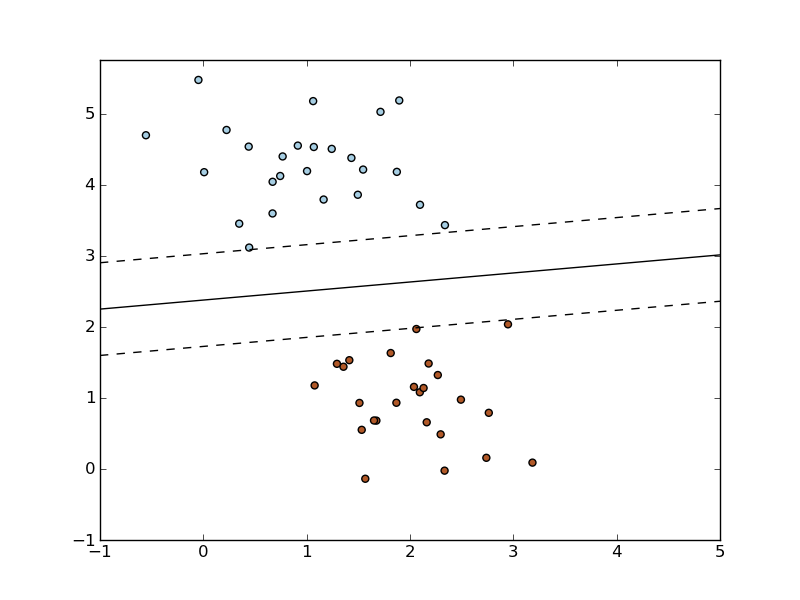
\includegraphics[width=.5\linewidth]{img/plot_sgd_separating_hyperplane_1.png}
    \caption{Example of SVC on toy problem}
\end{figure}

\subsection{Searchlight}

\begin{itemize}
    \item Present the Searchlight problem
    \item Say it is less a pain to implement thanks to scikit-learn bricks
        (estimator and cross\_val). Plus it is easily customizable.
\end{itemize}

\subsection{Classification of M/EEG sensor space data}


\subsection{Orthogonal Matching Pursuit}

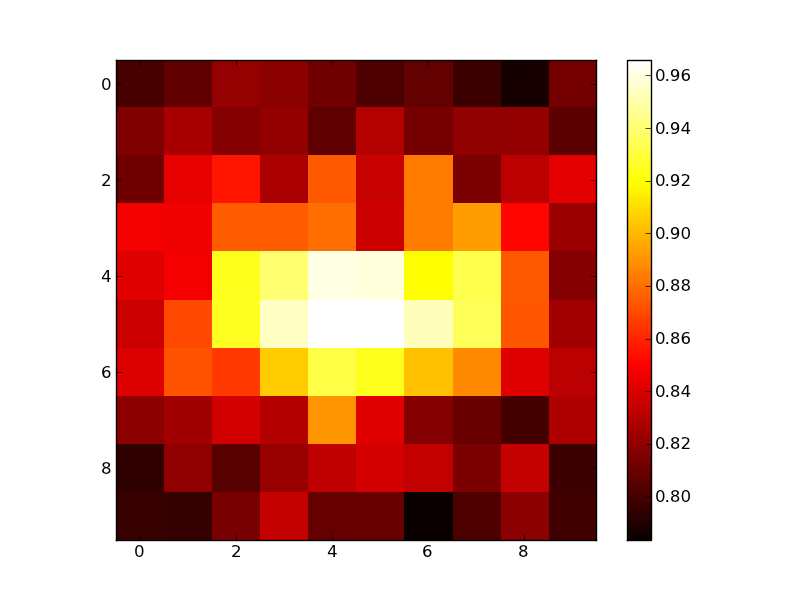
\includegraphics[width=.5\linewidth]{img/logistic_l1_scores.png}

\section{Encoding}

\alex{After talking with Michael, he told me that he could make a fairly simple
    example for encoding, which I think is a plus for the paper. The example will
    be integrated in Nisl.}

\section{Functional Connectivity}

\alex{Should we speak of correlation matrices to represent interaction between
regions?}

\subsection{ICA}

\begin{itemize}
    \item Explain principle
    \item Put several refs
    \item Put maps
    \item Should we talk about CANICA ?
\end{itemize}

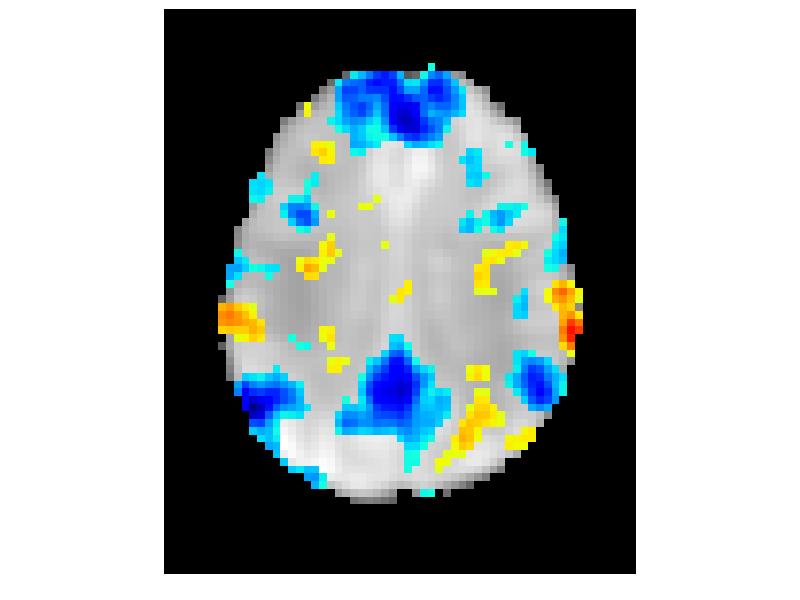
\includegraphics[width=.5\linewidth]{img/plot_canica_resting_state_17.png}

\subsection{Clustering}

Make  an  example  with   Ward   Clustering.  Indicate  then   that  other
algorithms  can  be  used  such  as
KMeans and Spectral clustering and only give results.

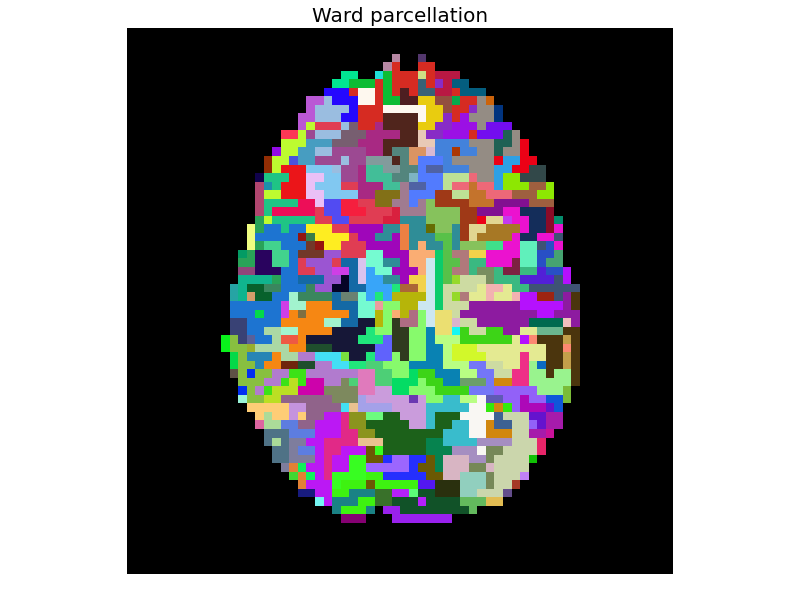
\includegraphics[width=.3\linewidth]{img/plot_rest_clustering_1.png}
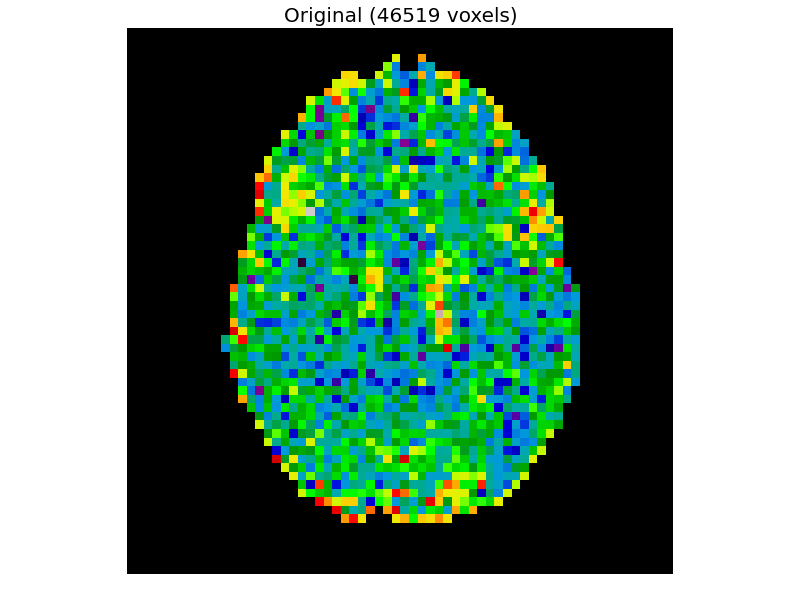
\includegraphics[width=.3\linewidth]{img/plot_rest_clustering_2.png}
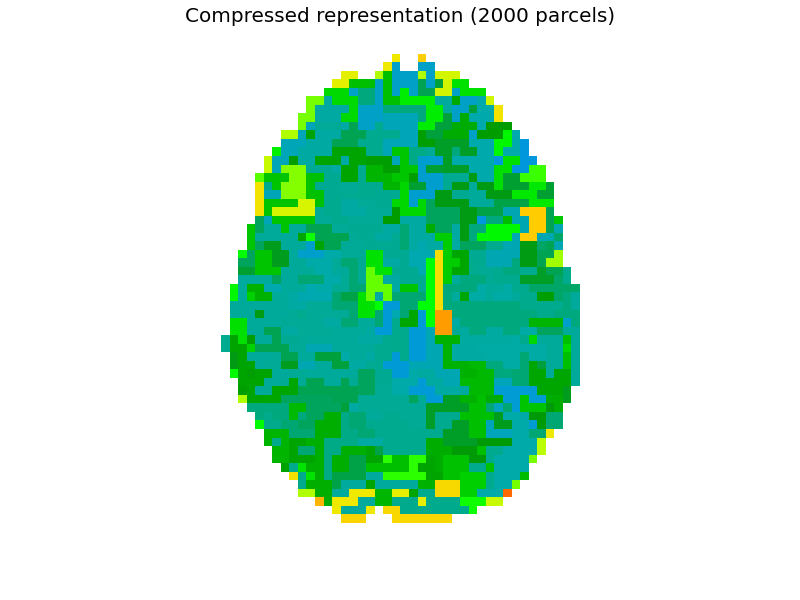
\includegraphics[width=.3\linewidth]{img/plot_rest_clustering_3.png}

\section{Data Sharing}

Frontiers supports the policy of data sharing, and authors are advised to make
freely available any materials and information described in their article, and
any data relevant to the article (while not compromising confidentiality in the
context of human-subject research) that may be reasonably requested by others
for the purpose of academic and non-commercial research. In regards to
deposition of data and data sharing through databases, Frontiers urges authors
to comply with the current best practices within their discipline.

\section*{Disclosure/Conflict-of-Interest Statement}
%All relationships financial, commercial or otherwise that might be perceived
%by the academic community as representing a potential conflict of interest
%must be described. If no such relationship exists, authors will be asked to
%declare that the research was conducted in the absence of any commercial or
%financial relationships that could be construed as a potential conflict of
%interest.
The authors declare that the research was conducted in the absence of any
commercial or financial relationships that could be construed as a potential
conflict of interest.

\section*{Acknowledgement} Text Text Text Text Text Text  Text Text Text Text
Text Text Text Text  Text Text Text Text Text Text Text Text Text  Text Text
Text.

\paragraph{Funding\textcolon} Text Text Text Text Text Text  Text Text.

\section*{Supplemental Data} Text Text Text Text Text Text  Text Text Text Text
Text Text Text Text Text  Text Text Text Text Text Text Text Text Text  Text
Text Text.

\bibliographystyle{frontiersinSCNS} % for Science articles
%\bibliographystyle{frontiersinMED} % for Medicine articles
\bibliography{test}

\end{document}
